\documentclass[tikz]{standalone}
\usepackage[outline]{contour}

\begin{document}
	    \contourlength{1.5pt}
	    	    \tikzset{
	    	double arrow/.style args={#1 colored by #2 and #3}{
	    		-stealth,line width=#1,#2, % first arrow
	    		postaction={draw,-stealth,#3,line width=(#1)/3,
	    			shorten <=(#1)/3,shorten >=2*(#1)/3}, % second arrow
	    	}
	    }
\begin{tikzpicture}
    \node[anchor=south west,inner sep=0] at (0,0) {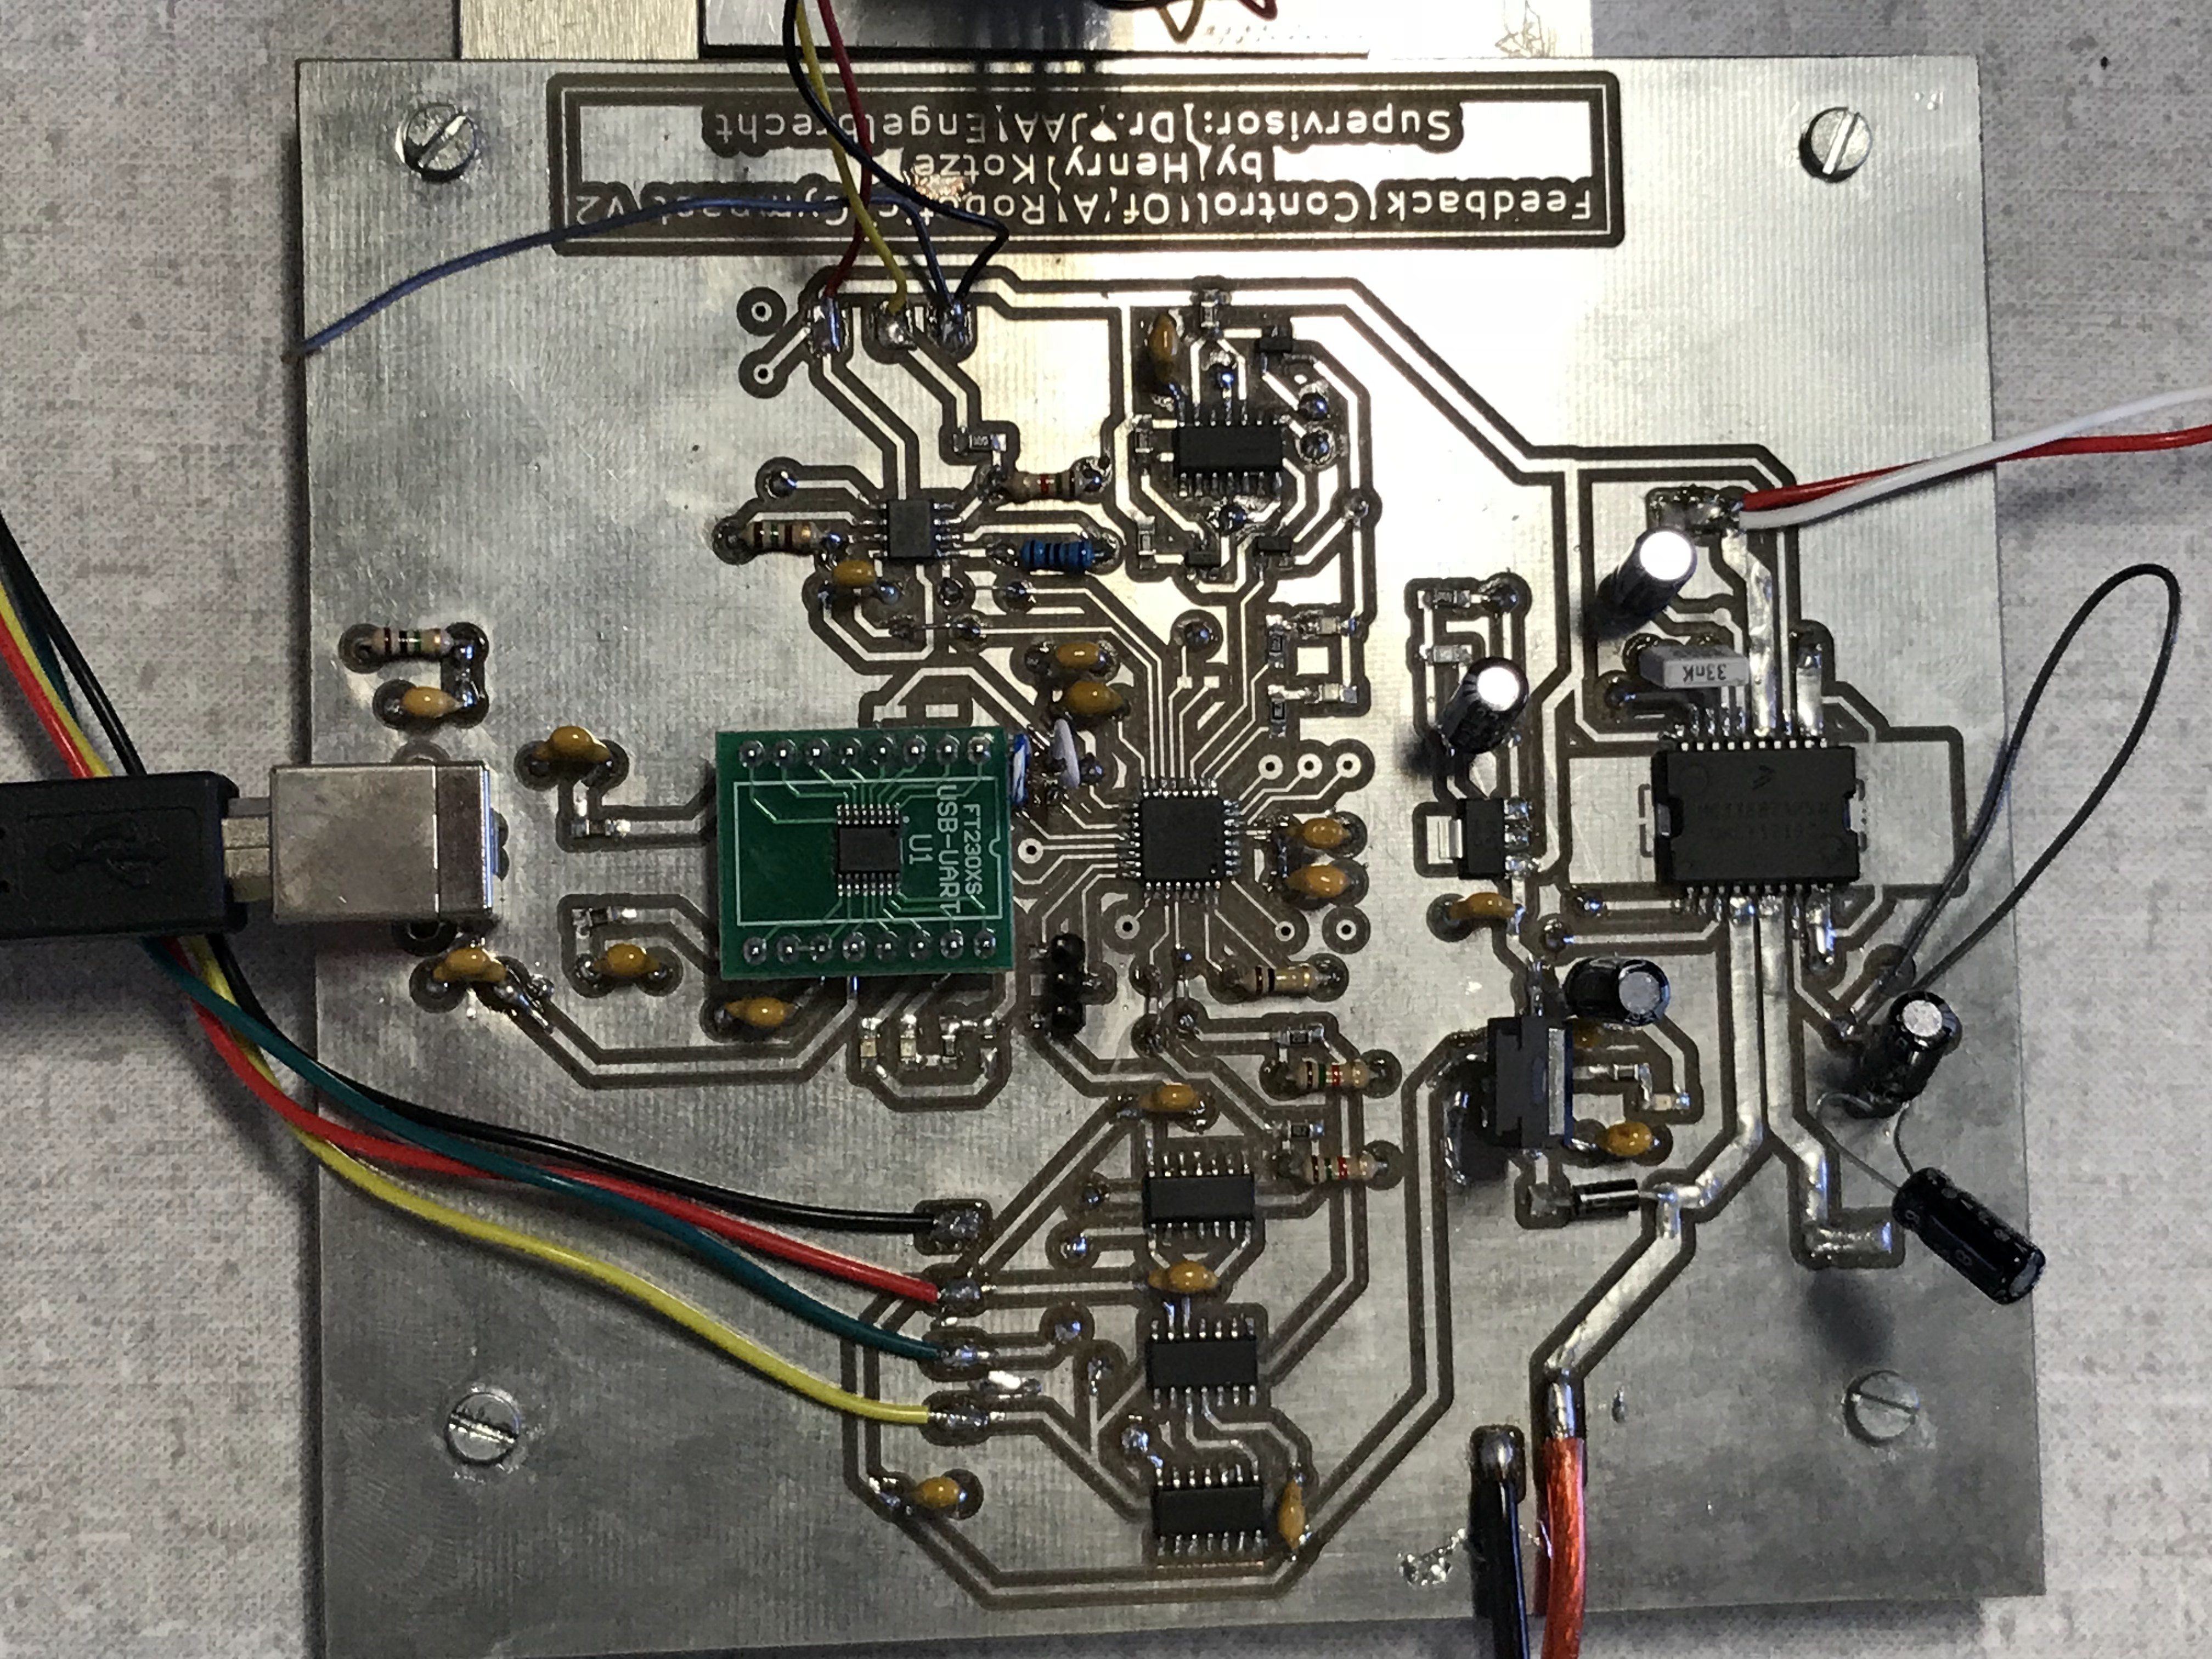
\includegraphics[width=\textwidth]{PCB.jpg}};
    %microcontroller
    %\draw[green,ultra thick,rounded corners] (6.5,5) node[above]{ \textbf{MCU} };
    

    
    \node[black] at (6.5,5.2) {\contour{white}{\textbf{MCU}}};
    
    \draw[yellow,ultra thick,rounded corners] (6,5) rectangle (7,4);
    
    %XOR
    \draw[yellow,ultra thick,rounded corners] (7.2,3) rectangle (6,0.5);
    \node[black] at (6.8,0.5) {\contour{white}{\textbf{XOR, NOR Digital Circuit}}};
    
    %UART
    \node[black] at (2.5,3.5) {\contour{white}{\textbf{UART}}};
    \draw[yellow,ultra thick,rounded corners] (1.5,3) rectangle (5.6,5.5);
    
    % AND
    \draw[yellow,ultra thick,rounded corners] (6,6) rectangle (7.5,7.5);
    \node[black] at (6.5,7.5) {\contour{white}{\textbf{AND Digital Circuit}}};
    
    %OPAMP
    \draw[yellow,ultra thick,rounded corners] (4,5.8) rectangle (5.5,6.5) ;
    \node[black] at (4.5,6.5) {\contour{white}{\textbf{Op-Amp}}};
    
    %REG
    \draw[yellow,ultra thick,rounded corners] (7.5,2.5) rectangle (8.8,6);
    \node[rotate=90,black] at (7.5,4.5) {\contour{white}{\textbf{Regulators}}};
    
    %Motor
    \draw[yellow,ultra thick,rounded corners] (9,2.5) rectangle (10.5,6);
    \node[rotate=90,black] at (10.5,4.5) {\contour{white}{\textbf{Motor Driver}}};
    
\end{tikzpicture}
\end{document}